%% This file was auto-generated by IPython, do NOT edit
%% Conversion from the original notebook file:
%% 02_Speeding_Python.ipynb
%%
\documentclass[11pt,english]{article}

%% This is the automatic preamble used by IPython.  Note that it does *not*
%% include a documentclass declaration, that is added at runtime to the overall
%% document.

\usepackage{amsmath}
\usepackage{amssymb}
\usepackage{graphicx}
\usepackage{ucs}
\usepackage[utf8x]{inputenc}

% needed for markdown enumerations to work
\usepackage{enumerate}

% Slightly bigger margins than the latex defaults
\usepackage{geometry}
\geometry{verbose,tmargin=3cm,bmargin=3cm,lmargin=2.5cm,rmargin=2.5cm}

% Define a few colors for use in code, links and cell shading
\usepackage{color}
\definecolor{orange}{cmyk}{0,0.4,0.8,0.2}
\definecolor{darkorange}{rgb}{.71,0.21,0.01}
\definecolor{darkgreen}{rgb}{.12,.54,.11}
\definecolor{myteal}{rgb}{.26, .44, .56}
\definecolor{gray}{gray}{0.45}
\definecolor{lightgray}{gray}{.95}
\definecolor{mediumgray}{gray}{.8}
\definecolor{inputbackground}{rgb}{.95, .95, .85}
\definecolor{outputbackground}{rgb}{.95, .95, .95}
\definecolor{traceback}{rgb}{1, .95, .95}

% Framed environments for code cells (inputs, outputs, errors, ...).  The
% various uses of \unskip (or not) at the end were fine-tuned by hand, so don't
% randomly change them unless you're sure of the effect it will have.
\usepackage{framed}

% remove extraneous vertical space in boxes
\setlength\fboxsep{0pt}

% codecell is the whole input+output set of blocks that a Code cell can
% generate.

% TODO: unfortunately, it seems that using a framed codecell environment breaks
% the ability of the frames inside of it to be broken across pages.  This
% causes at least the problem of having lots of empty space at the bottom of
% pages as new frames are moved to the next page, and if a single frame is too
% long to fit on a page, will completely stop latex from compiling the
% document.  So unless we figure out a solution to this, we'll have to instead
% leave the codecell env. as empty.  I'm keeping the original codecell
% definition here (a thin vertical bar) for reference, in case we find a
% solution to the page break issue.

%% \newenvironment{codecell}{%
%%     \def\FrameCommand{\color{mediumgray} \vrule width 1pt \hspace{5pt}}%
%%    \MakeFramed{\vspace{-0.5em}}}
%%  {\unskip\endMakeFramed}

% For now, make this a no-op...
\newenvironment{codecell}{}

 \newenvironment{codeinput}{%
   \def\FrameCommand{\colorbox{inputbackground}}%
   \MakeFramed{\advance\hsize-\width \FrameRestore}}
 {\unskip\endMakeFramed}

\newenvironment{codeoutput}{%
   \def\FrameCommand{\colorbox{outputbackground}}%
   \vspace{-1.4em}
   \MakeFramed{\advance\hsize-\width \FrameRestore}}
 {\unskip\medskip\endMakeFramed}

\newenvironment{traceback}{%
   \def\FrameCommand{\colorbox{traceback}}%
   \MakeFramed{\advance\hsize-\width \FrameRestore}}
 {\endMakeFramed}

% Use and configure listings package for nicely formatted code
\usepackage{listingsutf8}
\lstset{
  language=python,
  inputencoding=utf8x,
  extendedchars=\true,
  aboveskip=\smallskipamount,
  belowskip=\smallskipamount,
  xleftmargin=2mm,
  breaklines=true,
  basicstyle=\small \ttfamily,
  showstringspaces=false,
  keywordstyle=\color{blue}\bfseries,
  commentstyle=\color{myteal},
  stringstyle=\color{darkgreen},
  identifierstyle=\color{darkorange},
  columns=fullflexible,  % tighter character kerning, like verb
}

% The hyperref package gives us a pdf with properly built
% internal navigation ('pdf bookmarks' for the table of contents,
% internal cross-reference links, web links for URLs, etc.)
\usepackage{hyperref}
\hypersetup{
  breaklinks=true,  % so long urls are correctly broken across lines
  colorlinks=true,
  urlcolor=blue,
  linkcolor=darkorange,
  citecolor=darkgreen,
  }

% hardcode size of all verbatim environments to be a bit smaller
\makeatletter 
\g@addto@macro\@verbatim\small\topsep=0.5em\partopsep=0pt
\makeatother 

% Prevent overflowing lines due to urls and other hard-to-break entities.
\sloppy

\begin{document}

\begin{center}
{\bf Speeding Python}

{\bf \large Python in HPC}

{\bf TACC Training, Oct. 15, 2012}
\end{center}

\noindent Presenters:

\noindent {\bf Andy R. Terrel, PhD}\\
Texas Advanced Computing Center\\
University of Texas at Austin\\

\noindent {\bf Yaakoub El Khamra}\\
Texas Advanced Computing Center\\
University of Texas at Austin\\

\href{http://creativecommons.org/licenses/by/3.0/deed.en\_US}{\includegraphics{figures/creative_commons_logo.png}}\\

\noindent Python in HPC Tutorial by Terrel, and El Khamra is licensed
under a Creative Commons Attribution 3.0 Unported License. \\[2em]

\href{http://www.tacc.utexas.edu}{\includegraphics[scale=0.8]{figures/TACC_logo.png}} \qquad

\newpage


\newpage

\subsection{Interacting with the Tutorial Slides}

This tutorial is an interactive worksheet designed to encourage you to
try out the lessons during the demonstration. If you are looking at the
pdf version, we encourage you to download the updated version (see
previous slide) and try the interactive version.

To run the interactive version, you need a good Python environment
including:

\begin{itemize}
\item
  IPython version \textgreater{}= 13.0
\item
  Numpy version \textgreater{}= 1.5
\item
  Scipy
\item
  Matplotlib
\end{itemize}

Move to the directory containing the tarball and execute:

\begin{verbatim}
$ ipython notebook --pylab=inline
\end{verbatim}

We heartily endorse the
\href{https://store.continuum.io/cshop/anaconda}{Anaconda distribution}
and the \href{http://www.enthought.com/products/epd\_free.php}{Free
Enthought Python Distribution}.

\newpage

\subsection{Presentation mode}

 The slide show mode is only supported by an IPython development branch
version. To get it I recommend cloning from the official branch, adding
Matthias Carreau's remote, fetching and using his branch
slideshow\_extension2. Here are the commands:

\begin{verbatim}
git clone git://github.com/ipython/ipython.git # Official clone
cd ipython
git remote add carreau git://github.com/Carreau/ipython.git # Matthias' branch
git fetch carreau # Fetch the branches
git checkout carreau/slideshow_extension2 # Checkout the slideshow extension
python setup.py develop # Install the development version
ipython notebook # Check out the slideshows.
\end{verbatim}



\newpage

\section{How Slow is Python}

Let's add one to a million number

\begin{codecell}
\begin{codeinput}
\begin{lstlisting}
lst = range(1000000) # A pure Python list
%timeit [i + 1 for i in lst] # A Python list comprehension (iteration happens in C but with PyObjects)
\end{lstlisting}
\end{codeinput}
\begin{codeoutput}
\begin{verbatim}
10 loops, best of 3: 79.2 ms per loop
\end{verbatim}
\end{codeoutput}
\end{codecell}
\newpage

\subsection{Why is Python Slow?}

Dynamic typing requires lots of metadata around variable.

\begin{itemize}
\item
  Python uses heavy frame objects during iteration
\end{itemize}

\subsubsection{Solution:}

\begin{itemize}
\item
  Make an object that has a single type and continuous storage.
\item
  Implement common functionality into that object to iterate in C.
\end{itemize}

\begin{codecell}
\begin{codeinput}
\begin{lstlisting}
arr = arange(1000000) # A NumPy list of integers
%timeit arr + 1 # Use operator overloading for nice syntax, now iteration is in C with ints
\end{lstlisting}
\end{codeinput}
\begin{codeoutput}
\begin{verbatim}
100 loops, best of 3: 3.33 ms per loop
\end{verbatim}
\end{codeoutput}
\end{codecell}
\newpage

\subsection{What makes NumPy so much faster?}

\begin{itemize}
\item
  Data layout
\item
  homogenous: every item takes up the same size block of memory
\item
  single data-type objects
\item
  powerful array scalar types
\item
  universal function (ufuncs)
\item
  function that operates on ndarrays in an element-by-element fashion
\item
  vectorized wrapper for a function
\item
  built-in functions are implemented in compiled C code
\end{itemize}

\newpage

\subsection{Numpy Data layout}

\begin{itemize}
\item
  homogenous: every item takes up the same size block of memory
\item
  single data-type objects
\item
  powerful array scalar types
\end{itemize}

\begin{figure}[htbp]
\centering
\includegraphics{figures/numpy/threefundamental.png}
\caption{three fundamental}
\end{figure}

\newpage

\subsection{Numpy Universal Functions (ufuncs)}

\begin{itemize}
\item
  function that operates on ndarrays in an element-by-element fashion
\item
  vectorized wrapper for a function
\item
  built-in functions are implemented in compiled C code
\end{itemize}

\begin{codecell}
\begin{codeinput}
\begin{lstlisting}
%timeit [sin(i)**2 for i in arr]

\end{lstlisting}
\end{codeinput}
\begin{codeoutput}
\begin{verbatim}
1 loops, best of 3: 5.65 s per loop
\end{verbatim}
\end{codeoutput}
\end{codecell}
\begin{codecell}
\begin{codeinput}
\begin{lstlisting}
%timeit np.sin(arr)**2
\end{lstlisting}
\end{codeinput}
\begin{codeoutput}
\begin{verbatim}
10 loops, best of 3: 29.1 ms per loop
\end{verbatim}
\end{codeoutput}
\end{codecell}
\newpage

\subsection{Broadcasting Arrays}

Computing a 3D grid of distances $R_{ijk} = \sqrt(i^2 + j^2 + k^2)$

\begin{codecell}
\begin{codeinput}
\begin{lstlisting}
i, j, k = np.mgrid[-100:100, -100:100, -100:100]
print (i.shape, j.shape, k.shape)
\end{lstlisting}
\end{codeinput}
\begin{codeoutput}
\begin{verbatim}
((200, 200, 200), (200, 200, 200), (200, 200, 200))
\end{verbatim}
\end{codeoutput}
\end{codecell}
\begin{codecell}
\begin{codeinput}
\begin{lstlisting}
R = np.sqrt(i**2 + j**2 + k**2)
R.shape
\end{lstlisting}
\end{codeinput}
\begin{codeoutput}
\begin{verbatim}
(200, 200, 200)
\end{verbatim}
\end{codeoutput}
\end{codecell}
\begin{codecell}
\begin{codeinput}
\begin{lstlisting}
_ = imshow(R[100]/amax(R), cmap=cm.gray)
\end{lstlisting}
\end{codeinput}
\begin{codeoutput}
\begin{center}
\includegraphics[width=6in]{02_Speeding_Python_files/02_Speeding_Python_fig_00.png}
\par
\end{center}
\end{codeoutput}
\end{codecell}
\newpage

\subsection{Broadcasting Arrays}

But storing three dense arrays for a 3D grid is wasteful.

NumPy can broadcast across dimensions thus only working on the outer
grids

\begin{figure}[htbp]
\centering
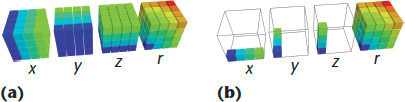
\includegraphics{figures/numpy_broadcast.png}
\caption{Numpy Broadcasting}
\end{figure}

\begin{codecell}
\begin{codeinput}
\begin{lstlisting}
i = arange(-100, 100).reshape(200, 1, 1)
j = reshape(i, (1, 200, 1))
k = reshape(i, (1, 1, 200))
R = np.sqrt(i**2 + j**2 + k**2)
\end{lstlisting}
\end{codeinput}
\end{codecell}
\begin{codecell}
\begin{codeinput}
\begin{lstlisting}
_ = pcolor(R[-50]/amax(R))
\end{lstlisting}
\end{codeinput}
\begin{codeoutput}
\begin{center}
\includegraphics[width=6in]{02_Speeding_Python_files/02_Speeding_Python_fig_01.png}
\par
\end{center}
\end{codeoutput}
\end{codecell}
\begin{codecell}
\begin{codeinput}
\begin{lstlisting}
i, j, k = ogrid[-100:100, -100:100, -100:100]
R = np.sqrt(i**2 + j**2 + k**2)
\end{lstlisting}
\end{codeinput}
\end{codecell}
\newpage

\subsection{NumPy's View of Data}

\begin{codecell}
\begin{codeinput}
\begin{lstlisting}
print array([1,2,3], dtype=float)
print arange(10).astype(float)
print np.int8(arange(10, dtype=float))
print np.dtype(int)
print np.issubdtype(np.int32, np.int)
print np.issubdtype(np.int, np.float)
\end{lstlisting}
\end{codeinput}
\begin{codeoutput}
\begin{verbatim}
[ 1.  2.  3.]
[ 0.  1.  2.  3.  4.  5.  6.  7.  8.  9.]
[0 1 2 3 4 5 6 7 8 9]
int64
True
False
\end{verbatim}
\end{codeoutput}
\end{codecell}
\newpage

\subsection{Arrays of Structs in NumPy}

\begin{codecell}
\begin{codeinput}
\begin{lstlisting}
x = np.zeros((2,),dtype=('i4,f4,a10')) 
print x
\end{lstlisting}
\end{codeinput}
\begin{codeoutput}
\begin{verbatim}
[(0, 0.0, '') (0, 0.0, '')]
\end{verbatim}
\end{codeoutput}
\end{codecell}
\begin{codecell}
\begin{codeinput}
\begin{lstlisting}
x[:] = [(1,2.,'Hello'),(2,3.,"World")]
print x
\end{lstlisting}
\end{codeinput}
\begin{codeoutput}
\begin{verbatim}
[(1, 2.0, 'Hello') (2, 3.0, 'World')]
\end{verbatim}
\end{codeoutput}
\end{codecell}
\begin{codecell}
\begin{codeinput}
\begin{lstlisting}
dt = dtype([('time', uint64),
            ('pos', [
               ('x', float),
               ('y', float)])])
x = np.array([
        (100, ( 0, 0.5)),
        (200, ( 0, 10.3)),
        (300, (5.5, 15.1))],
        dtype=dt)
print x['time']
print x[ x['time'] >= 200 ]
\end{lstlisting}
\end{codeinput}
\begin{codeoutput}
\begin{verbatim}
[100 200 300]
[(200L, (0.0, 10.3)) (300L, (5.5, 15.1))]
\end{verbatim}
\end{codeoutput}
\end{codecell}
\newpage

\section{Profiling Python}

Profiling is an important way to find the bottlenecks in a program.
Python has several different profilers, here we show the most common one
that is part of the standard library.

\begin{codecell}
\begin{codeinput}
\begin{lstlisting}
def mandelbrot (x, y, maxit):
    c = x + y*1.j
    z = 0. + 0.j
    it = 0
    while abs(z) < 2 and it < maxit:
        z = z**2 + c
        it += 1
    return float(it)/maxit

def draw_mandelbrot(num_x, num_y):
    results = []
    for x in linspace(-2.0, 1.0, num_x):
        results.append([])
        for y in linspace(-1.0, 1.0, num_y):
            results[-1].append(mandelbrot(x, y, 10))
    imshow(results)
    
draw_mandelbrot(100,100)
\end{lstlisting}
\end{codeinput}
\begin{codeoutput}
\begin{center}
\includegraphics[width=6in]{02_Speeding_Python_files/02_Speeding_Python_fig_02.png}
\par
\end{center}
\end{codeoutput}
\end{codecell}
\begin{codecell}
\begin{codeinput}
\begin{lstlisting}
import profile
profile.run("draw_mandelbrot(10, 10)", "dm.stats")
\end{lstlisting}
\end{codeinput}
\begin{codeoutput}
\begin{center}
\includegraphics[width=6in]{02_Speeding_Python_files/02_Speeding_Python_fig_03.png}
\par
\end{center}
\end{codeoutput}
\end{codecell}
\begin{codecell}
\begin{codeinput}
\begin{lstlisting}
import pstats
p = pstats.Stats('dm.stats')
p.strip_dirs().sort_stats(-1).print_stats(10)
\end{lstlisting}
\end{codeinput}
\begin{codeoutput}
\begin{verbatim}
Sat Oct 13 22:47:21 2012    dm.stats

         34798 function calls (34263 primitive calls) in 0.352 seconds

   Ordered by: standard name
   List reduced from 418 to 10 due to restriction <10>

   ncalls  tottime  percall  cumtime  percall filename:lineno(function)
      654    0.003    0.000    0.003    0.000 :0(abs)
        2    0.000    0.000    0.000    0.000 :0(accumulate)
      585    0.008    0.000    0.008    0.000 :0(all)
        1    0.000    0.000    0.000    0.000 :0(any)
      249    0.001    0.000    0.001    0.000 :0(append)
       13    0.000    0.000    0.000    0.000 :0(arange)
     1298    0.018    0.000    0.018    0.000 :0(array)
       80    0.000    0.000    0.000    0.000 :0(callable)
        1    0.000    0.000    0.000    0.000 :0(can_cast)
       40    0.001    0.000    0.001    0.000 :0(concatenate)
\end{verbatim}
\begin{verbatim}
<pstats.Stats instance at 0x1114f05f0>
\end{verbatim}
\end{codeoutput}
\end{codecell}
\begin{codecell}
\begin{codeinput}
\begin{lstlisting}
p.strip_dirs().sort_stats('time').print_stats(10)
\end{lstlisting}
\end{codeinput}
\begin{codeoutput}
\begin{verbatim}
Sat Oct 13 22:47:21 2012    dm.stats

         34798 function calls (34263 primitive calls) in 0.352 seconds

   Ordered by: internal time
   List reduced from 418 to 10 due to restriction <10>

   ncalls  tottime  percall  cumtime  percall filename:lineno(function)
      585    0.024    0.000    0.055    0.000 path.py:86(__init__)
     1298    0.018    0.000    0.018    0.000 :0(array)
      120    0.018    0.000    0.167    0.001 lines.py:128(__init__)
      540    0.013    0.000    0.117    0.000 markers.py:115(_recache)
     2544    0.012    0.000    0.012    0.000 __init__.py:662(__getitem__)
     1145    0.011    0.000    0.018    0.000 transforms.py:80(__init__)
     2101    0.009    0.000    0.009    0.000 :0(isinstance)
      100    0.009    0.000    0.011    0.000 <ipython-input-15-036d85cb27e4>:1(mandelbrot)
      933    0.008    0.000    0.022    0.000 transforms.py:1321(__init__)
      983    0.008    0.000    0.016    0.000 numeric.py:167(asarray)
\end{verbatim}
\begin{verbatim}
<pstats.Stats instance at 0x1114f05f0>
\end{verbatim}
\end{codeoutput}
\end{codecell}
\begin{codecell}
\begin{codeinput}
\begin{lstlisting}
def draw_mandelbrot2(num_x, num_y):
    results = np.zeros((num_x+1, num_y+1), dtype=float)
    for i,x in enumerate(linspace(-2.0, 1.0, num_x)):
        for j,y in enumerate(linspace(-1.0, 1.0, num_y)):
            results[i, j] = mandelbrot(x, y, 100)
    imshow(results, cmap=cm.coolwarm)
draw_mandelbrot2(100,100)
\end{lstlisting}
\end{codeinput}
\begin{codeoutput}
\begin{center}
\includegraphics[width=6in]{02_Speeding_Python_files/02_Speeding_Python_fig_04.png}
\par
\end{center}
\end{codeoutput}
\end{codecell}
\begin{codecell}
\begin{codeinput}
\begin{lstlisting}
profile.run("draw_mandelbrot2(10, 10)", "dm2.stats")
\end{lstlisting}
\end{codeinput}
\begin{codeoutput}
\begin{center}
\includegraphics[width=6in]{02_Speeding_Python_files/02_Speeding_Python_fig_05.png}
\par
\end{center}
\end{codeoutput}
\end{codecell}
\begin{codecell}
\begin{codeinput}
\begin{lstlisting}
p = pstats.Stats('dm2.stats')
p.strip_dirs().sort_stats(-1).print_stats(10)
\end{lstlisting}
\end{codeinput}
\begin{codeoutput}
\begin{verbatim}
Sat Oct 13 22:47:24 2012    dm2.stats

         36976 function calls (36441 primitive calls) in 0.363 seconds

   Ordered by: standard name
   List reduced from 418 to 10 due to restriction <10>

   ncalls  tottime  percall  cumtime  percall filename:lineno(function)
     2944    0.013    0.000    0.013    0.000 :0(abs)
        2    0.000    0.000    0.000    0.000 :0(accumulate)
      585    0.007    0.000    0.007    0.000 :0(all)
        1    0.000    0.000    0.000    0.000 :0(any)
      139    0.000    0.000    0.000    0.000 :0(append)
       13    0.000    0.000    0.000    0.000 :0(arange)
     1298    0.016    0.000    0.016    0.000 :0(array)
       80    0.000    0.000    0.000    0.000 :0(callable)
        1    0.000    0.000    0.000    0.000 :0(can_cast)
       40    0.001    0.000    0.001    0.000 :0(concatenate)
\end{verbatim}
\begin{verbatim}
<pstats.Stats instance at 0x1293fb5a8>
\end{verbatim}
\end{codeoutput}
\end{codecell}
\newpage

\section{Compiling to C}

C is faster, and Python is easier to write. We want both!

\subsection{Cython}

\begin{itemize}
\item
  a programming language based on Python
\item
  uses extra syntax allowing for optional static type declarations
\item
  source code gets translated into optimized C/C++ code and compiled as
  Python extension modules
\end{itemize}

\newpage

\subsection{Using Cython in IPython}

In IPython we can make any cell call out to Cython via the cell magic

First load the extension

\begin{codecell}
\begin{codeinput}
\begin{lstlisting}
%load_ext cythonmagic
\end{lstlisting}
\end{codeinput}
\end{codecell}
Now use \texttt{\%\%cython} at the begining of a code cell to call out
to Cython.

\begin{codecell}
\begin{codeinput}
\begin{lstlisting}
%%cython
def f_cython(int i):
    return i**4 + 3*i**2 + 10
\end{lstlisting}
\end{codeinput}
\end{codecell}
Now use Cython function in code:

\begin{codecell}
\begin{codeinput}
\begin{lstlisting}
f_cython(100)
\end{lstlisting}
\end{codeinput}
\begin{codeoutput}
\begin{verbatim}
100030010
\end{verbatim}
\end{codeoutput}
\end{codecell}
\newpage

\subsection{How much faster is Cython?}

The more you are able to provide type information the better the
compile. For example f without type information:

\begin{codecell}
\begin{codeinput}
\begin{lstlisting}
def f_python(i):
    return i**4 + 3*i**2 + 10
\end{lstlisting}
\end{codeinput}
\end{codecell}
\begin{codecell}
\begin{codeinput}
\begin{lstlisting}
%timeit f_python(100)
\end{lstlisting}
\end{codeinput}
\begin{codeoutput}
\begin{verbatim}
1000000 loops, best of 3: 409 ns per loop
\end{verbatim}
\end{codeoutput}
\end{codecell}
\begin{codecell}
\begin{codeinput}
\begin{lstlisting}
%timeit f_cython(100)
\end{lstlisting}
\end{codeinput}
\begin{codeoutput}
\begin{verbatim}
10000000 loops, best of 3: 114 ns per loop
\end{verbatim}
\end{codeoutput}
\end{codecell}
\newpage

\subsection{Declaring Cython variables for C level}

If you use a variable or function only at the Cython level you can keep
it in C via \texttt{cdef}:

\begin{codecell}
\begin{codeinput}
\begin{lstlisting}
%%cython
cdef f(double x):
    return x**2-x

def integrate_f(double a, double b, int N):
    cdef int i
    cdef double s, dx
    s = 0
    dx = (b-a)/N
    for i in range(N):
        s += f(a+i*dx)
    return s * dx
\end{lstlisting}
\end{codeinput}
\end{codecell}
\begin{codecell}
\begin{codeinput}
\begin{lstlisting}
%timeit integrate_f(1.0, 2.0, 1000)
\end{lstlisting}
\end{codeinput}
\begin{codeoutput}
\begin{verbatim}
10000 loops, best of 3: 36.6 us per loop
\end{verbatim}
\end{codeoutput}
\end{codecell}
The pure Python version:

\begin{codecell}
\begin{codeinput}
\begin{lstlisting}
def f(x):
    return x**2-x

def integrate_f(a, b, N):
    s = 0
    dx = (b-a)/N
    for i in range(N):
        s += f(a+i*dx)
    return s * dx
\end{lstlisting}
\end{codeinput}
\end{codecell}
\begin{codecell}
\begin{codeinput}
\begin{lstlisting}
%timeit integrate_f(1.0, 2.0, 1000)
\end{lstlisting}
\end{codeinput}
\begin{codeoutput}
\begin{verbatim}
1000 loops, best of 3: 498 us per loop
\end{verbatim}
\end{codeoutput}
\end{codecell}
\newpage

\subsection{Using NumPy with Cython}

You can also use fast accessors to NumPy arrays from Cython:

\begin{codecell}
\begin{codeinput}
\begin{lstlisting}
%%cython
import numpy as np
# "cimport" is used to import special compile-time information
# about the numpy module (this is stored in a file numpy.pxd which is
# currently part of the Cython distribution).
cimport numpy as np
# We now need to fix a datatype for our arrays. I've used the variable
# DTYPE for this, which is assigned to the usual NumPy runtime
# type info object.
DTYPE = np.int
# "ctypedef" assigns a corresponding compile-time type to DTYPE_t. For
# every type in the numpy module there's a corresponding compile-time
# type with a _t-suffix.
ctypedef np.int_t DTYPE_t
# "def" can type its arguments but not have a return type. The type of the
# arguments for a "def" function is checked at run-time when entering the
# function.
#
# The arrays f, g and h is typed as "np.ndarray" instances. The only effect
# this has is to a) insert checks that the function arguments really are
# NumPy arrays, and b) make some attribute access like f.shape[0] much
# more efficient. (In this example this doesn't matter though.)
def naive_convolve(np.ndarray f, np.ndarray g):
    if g.shape[0] % 2 != 1 or g.shape[1] % 2 != 1:
        raise ValueError("Only odd dimensions on filter supported")
    assert f.dtype == DTYPE and g.dtype == DTYPE
    # The "cdef" keyword is also used within functions to type variables. It
    # can only be used at the top indendation level (there are non-trivial
    # problems with allowing them in other places, though we'd love to see
    # good and thought out proposals for it).
    #
    # For the indices, the "int" type is used. This corresponds to a C int,
    # other C types (like "unsigned int") could have been used instead.
    # Purists could use "Py_ssize_t" which is the proper Python type for
    # array indices.
    cdef int vmax = f.shape[0]
    cdef int wmax = f.shape[1]
    cdef int smax = g.shape[0]
    cdef int tmax = g.shape[1]
    cdef int smid = smax // 2
    cdef int tmid = tmax // 2
    cdef int xmax = vmax + 2*smid
    cdef int ymax = wmax + 2*tmid
    cdef np.ndarray h = np.zeros([xmax, ymax], dtype=DTYPE)
    cdef int x, y, s, t, v, w
    # It is very important to type ALL your variables. You do not get any
    # warnings if not, only much slower code (they are implicitly typed as
    # Python objects).
    cdef int s_from, s_to, t_from, t_to
    # For the value variable, we want to use the same data type as is
    # stored in the array, so we use "DTYPE_t" as defined above.
    # NB! An important side-effect of this is that if "value" overflows its
    # datatype size, it will simply wrap around like in C, rather than raise
    # an error like in Python.
    cdef DTYPE_t value
    for x in range(xmax):
        for y in range(ymax):
            s_from = max(smid - x, -smid)
            s_to = min((xmax - x) - smid, smid + 1)
            t_from = max(tmid - y, -tmid)
            t_to = min((ymax - y) - tmid, tmid + 1)
            value = 0
            for s in range(s_from, s_to):
                for t in range(t_from, t_to):
                    v = x - smid + s
                    w = y - tmid + t
                    value += g[smid - s, tmid - t] * f[v, w]
            h[x, y] = value
    return h
\end{lstlisting}
\end{codeinput}
\end{codecell}
\begin{codecell}
\begin{codeinput}
\begin{lstlisting}
N=100
f = np.arange(N*N, dtype=np.int).reshape((N,N))
g = np.arange(81, dtype=np.int).reshape((9, 9))
%timeit -n2 -r3 naive_convolve(f, g)
\end{lstlisting}
\end{codeinput}
\begin{codeoutput}
\begin{verbatim}
2 loops, best of 3: 1.62 s per loop
\end{verbatim}
\end{codeoutput}
\end{codecell}
\end{document}
